\documentclass[11pt,fleqn]{article}

\setlength {\topmargin} {-.15in}
\setlength {\textheight} {8.6in}

\usepackage{amsmath}
\usepackage{amssymb}
\usepackage{color}
\usepackage{tikz}
\usetikzlibrary{automata,positioning,arrows}
\usepackage{diagbox}
\usepackage{stackrel}
\begin{document}


\textbf{Exercise 1.4.15:} Faster 3-sum. As a warmup, develop an implementation TwoSumFaster that
uses a $linear$ algorithm to count the pairs that sum to zero after the array is sorted ($instead$
$of$ the binary-search-based $linearithmic$ algorithm). Then apply a similar idea to
develop a $quadratic$ algorithm for the 3-sum problem.\\

\textbf{Solution:}
\begin{center}
	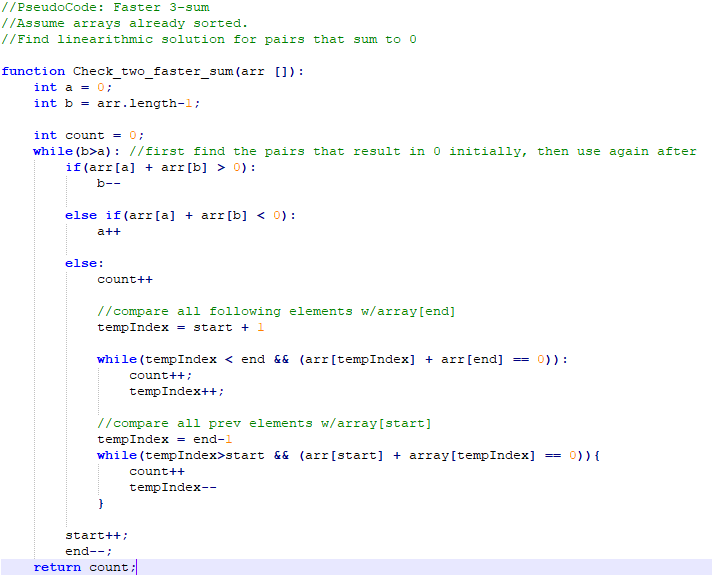
\includegraphics[scale = 1]{1.4.15-code.png}
	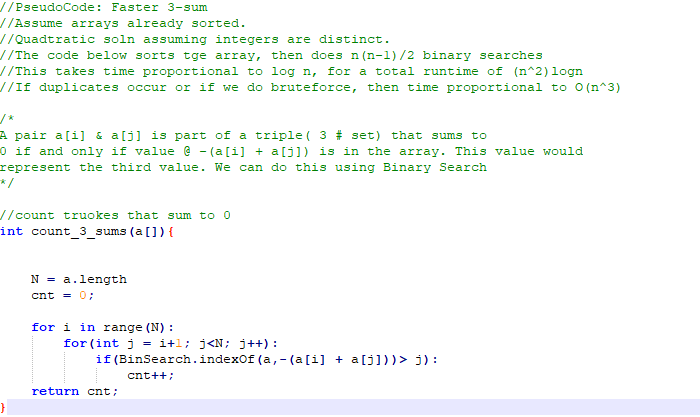
\includegraphics[scale = 1]{1.4.15-code2.png}
	\end{center}

\end{document}
